\chapter{Interpretação dos resultados}

Neste capítulo, será abordado a interpretação dos resultados obtidos durante durante a implementação dos códigos e solução dos problemas. Serão analisados os resultados obtidos, relacionando-os com a metodologia e verificando a coerência dos resultados com os fenômenos físicos esperados. 

\section{Cálculo da gravidade de planeta axis simétrico}


O primeiro problema, trata-se da comparação entre os modelos de gravidade para planeta axis simétrico e esférico. As componentes gravitacionais são $g_r$ que está na direção do centro do planeta, porém seu sentido é para fora dele, e $g_{\phi}$ que aponta para o norte no planeta. Os gráficos são representados da forma que $h = 200 km$ quando $\delta = 100 \degree$ e $h = 0 km$ quando $\delta = -100\degree$.

\begin{figure}[H]
\centering
\caption{Comparação entre as componentes da gravidade para um planeta esférico e um axis simétrico.}
\label{fig: Exemplo 3.1}
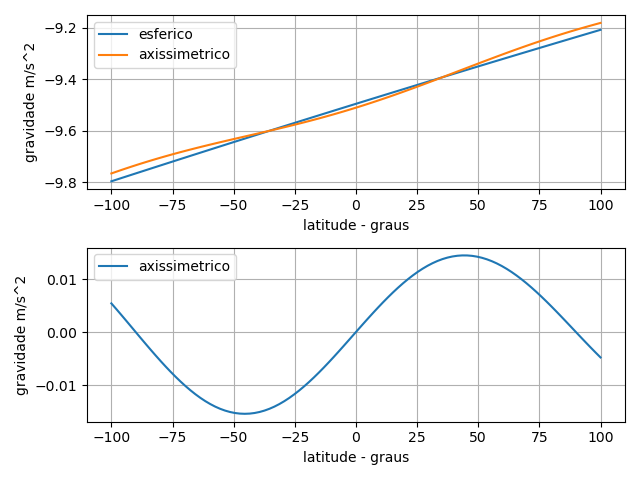
\includegraphics[width=0.8\textwidth]{figuras/Resultados/exemplo31.png}
\fonte{Autores, 2023}
\end{figure}

Observa-se que a componente $g_r$ é igual para ambos os modelos quando a latitude é igual a $\pm 45\degree$ e a componente $g_{\phi}$ é igual no equador e nos polos. A maior diferença entre os modelos pode ser observado para $g_r$ nos polos e para $g_{\phi}$ quando $\delta = \pm 45 \degree$. Ainda, nota-se que a magnitude dessas variações não é tão grande, porém pode gerar um erro gigantesco em simulações de voos de longa duração, praticamente a totalidade das operações aeroespaciais.

\section{Propagação de órbita}

A propagação de órbita permite prever com precisão a posição futura de um objeto em órbita, o que é fundamental para o planejamento de missões espaciais, manobras orbitais, posicionamento de satélites e controle de espaçonaves. Além disso, a propagação de órbita também é utilizada para monitorar o estado de saúde de satélites em órbita, detectar possíveis colisões e realizar ajustes necessários para manter a órbita desejada. Serão apresentadas 3 tipos de órbitas: elíptica; hiperbólica e parabólica, sendo apresentadas as variações da anomalia verdadeira, $\theta$, componente da velocidade na direção x, $v_x$,componente da velocidade na direção y, $v_y$ no tempo, e as coordenadas no plano $XY$.

\subsection{Órbita elíptica}

Uma órbita elíptica é caracterizada por ter a forma de uma elipse. Nesse tipo de órbita, o objeto em movimento descreve uma trajetória oval ao redor do corpo celeste central, como a Terra. A elipse possui dois focos, sendo que o corpo celeste central (como a Terra) está localizado em um dos focos. A figura \ref{fig: Resultado - Propagação de órbita elíptica}, mostra as variações dos parâmetros para esse tipo de órbita. Ainda é considerado o a variação da anomalia excêntrica.

\begin{figure}[H]
\centering
\caption{Propagação de órbita elíptica.}
\label{fig: Resultado - Propagação de órbita elíptica}
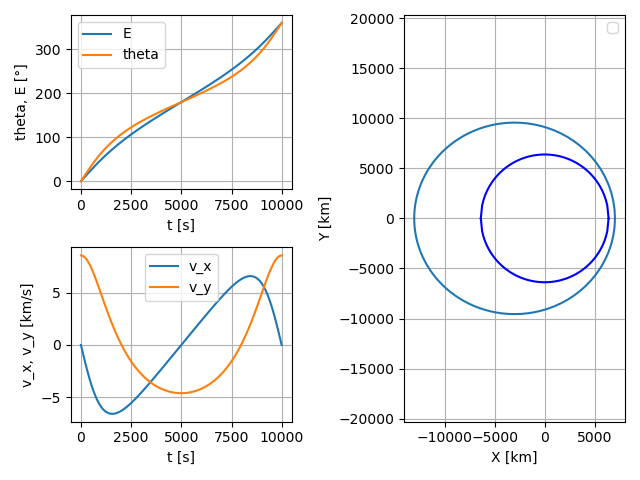
\includegraphics[width=0.8\textwidth]{figuras/Resultados/aula6_eliptica.png}
\fonte{Autores, 2023}
\end{figure}

Como esperado, para a órbita elíptica, a anomalia verdadeira deverá ser igual a anomalia excêntrica nos pontos em que $\theta = n\pi$, para $n$ inteiro, isso ocorre devido ao fato que no periastro e no apoastro as anomalias excêntrica e verdadeira coincidem. Também observa-se que as componentes da velocidade estão coerentes pois $v_x = 0$ quando $v_y = max$, porém o contrário não é válido justamente pelas características da órbita, seria válido apenas para uma órbita circular. Por último o gráfico mais a direita mostra o formato elíptico da órbita.

\subsection{Órbita hiperbólica}

Uma órbita hiperbólica é caracterizada por ter a forma de uma hipérbole. Nesse tipo de órbita, o objeto em movimento descreve uma trajetória aberta, em forma de "U". A velocidade do objeto em relação ao corpo celeste central é suficientemente alta para que ele escape da influência gravitacional e não retorne. Essas órbitas são utilizadas para missões espaciais interplanetárias ou quando se deseja realizar uma trajetória de passagem próxima a um corpo celeste sem entrar em órbita. Para essa órbita também é observado a variação da anomalia hiperbólica.

\begin{figure}[H]
\centering
\caption{Propagação de órbita hiperbólica.}
\label{fig: Resultado - Propagação de órbita hiperbólica}
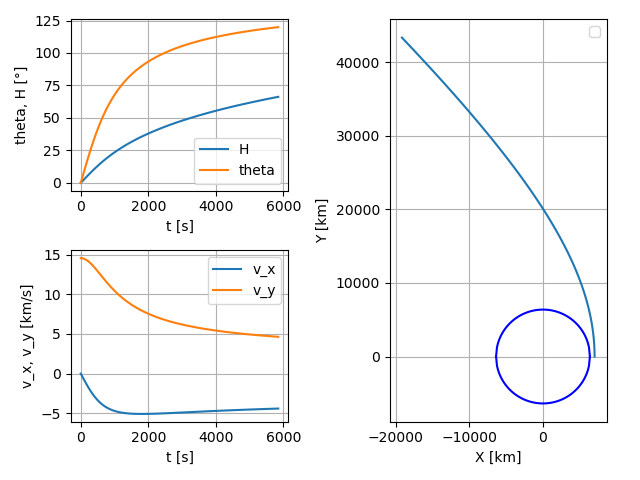
\includegraphics[width=0.8\textwidth]{figuras/Resultados/aula6_hiperbolica.png}
\fonte{Autores, 2023}
\end{figure}

Por se tratar de uma órbita de escape, não existe uma repetição de valores das velocidades como para a órbita elíptica, eles tendem a convergir para algum valor conforme pode ser observado pela figura \ref{fig: Resultado - Propagação de órbita hiperbólica}. Para a anomalia verdadeira, observa-se uma mudança rápida em seu valor e depois um amortecimento fazendo ela tender a um valor, o que também faz sentido por se tratar de uma órbita de escape. Ainda, a anomalia hiperbólica tem sua magnitude menor que a anomalia verdadeira, o que também está coerente já que ela está relacionada a uma função hiperbólica. Por ultimo o gráfico da trajetória representa a forma hiperbólica da trajetória e mostrando a sua posição tendendo para longe da órbita circular.

\subsection{Órbita parabólica}

Uma órbita parabólica é uma órbita especial que está no limite entre as órbitas elípticas e hiperbólicas. Nesse tipo de órbita, o objeto em movimento descreve uma trajetória parabólica. A velocidade do objeto é exatamente suficiente para que ele escape da influência gravitacional do corpo celeste central, mas sem energia cinética adicional para se afastar indefinidamente. Essas órbitas são raras e geralmente ocorrem em situações especiais, como trajetórias de passagem próxima a um corpo celeste ou quando a velocidade de lançamento é cuidadosamente ajustada.

\begin{figure}[H]
\centering
\caption{Propagação de órbita parabólica.}
\label{fig: Resultado - Propagação de órbita parabólica}
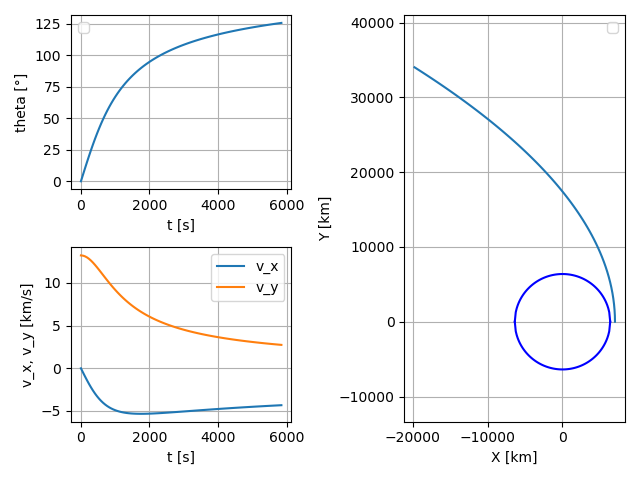
\includegraphics[width=0.8\textwidth]{figuras/Resultados/aula6_parabolica.png}
\fonte{Autores, 2023}
\end{figure}

Da mesma forma que para a órbita hiperbólica, a órbita parabólica é de escape e pode ser observado na figura \ref{fig: Resultado - Propagação de órbita parabólica}. Tanto as componentes da velocidade quanto a anomalia verdadeira são bem parecidas com a órbita hiperbólica o que é bem coerente.

\section{Determinação de órbita}
\par Nessa seção será resolvido um exemplo onde serão obtidos os parâmetros de uma órbita em um problema de dois corpos a partir de uma única observação de posição e velocidade. Os elementos orbitais consistem em 6 parâmetros, que descrevem a progressão e a orientação da órbita. Um conjunto comum de elementos orbitais inclui a excentricidade, semi eixo maior, tempo de periastro, longitude celeste do nodo ascendente, inclinação e argumento de periastro. 
\par Do enunciado tem-se que uma espaçonave observada no referencial centrado na Terra possui a seguinte posição e velocidade celeste: \textbf{r}=-500\textbf{I}+12500\textbf{K} [km] e \textbf{v}=5\textbf{I}-8\textbf{J}[km/s]. Foi solicitado que fosse determinado os parâmetros orbitais. Utilizando o programa desenvolvido em aula, foram obtidos os valores mostrados na tabela \ref{ex52}

\begin{table}[H]
\centering
\caption{Resultados Exemplo 5.2 -Determinação de Órbita}
\begin{tabular}{|c|c|c|}
\hline
Elementos Orbitais & Valor               & Unidade \\ \hline
Semi-Eixo Maior          & -13382.403826218939 & Km      \\ \hline
Excentricidade          & 1.9765961447821856  & - \\ \hline
$\tau$        & 416.7937786907604   & s       \\ \hline
$\Omega$      & 122.0053832080835   & graus   \\ \hline
i          & 71.26309861909091   & graus   \\ \hline
$\omega$      & 95.71519588364482   & graus   \\ \hline
\end{tabular}
\label{ex52}
\end{table}

\par Analisando os elementos pode-se afirmar que a espaçonave se aproxima da Terra, uma vez que $\tau$ é positivo. Isso também pode ser visto devido a anomalia verdadeira no quarto quadrante.

\nocite{book:226549}

\section{Manobras orbitais}

\par As manobras orbitais desempenham um papel crucial na exploração espacial e na operação de satélites, permitindo que espaçonaves e satélites alterem sua posição, velocidade e direção no espaço. Essas manobras são essenciais para alcançar órbitas desejadas, manter a estabilidade orbital, evitar colisões e realizar missões específicas. \par Para uma maior compreensão do assunto e aplicação dos conceitos vistos anteriormente serão discutidos os resultados dos exemplos mostrados a seguir.

\subsection{Exemplo 5.6}

\par É dado que um veículo espacial está em uma órbita terrestre de altitude 500 km, com inclinação de 10\degree , deve ser enviado para uma órbita elíptica com altitudes de perigeu de 200km e apogeu de 700km, bem como inclinação de 5\degree. 
\par Serão aplicados dois impulsos; um para a obtenção da órbita elíptica e o segundo para mudar a inclinação da orbita intermediária, sendo que esse é aplicado no apogeu para minimizar a quantidade de propelente. 
\par O primeiro impulso deve ser aplicado com um ângulo $\beta_1$, uma vez que a altitude de perigeu solicitada é diferente da inicial. Este está relacionado com a velocidade inicial e final.

\par O segundo impulso de velocidade é baseado na variação de inclinação necessária. Da mesma forma, esse deve ser aplicado de formar a minimizar o uso de propelente, isso se dá com a aplicação no apogeu. 

\par Com essas considerações e utilizando o programa desenvolvido em aula, obtém-se os seguintes resultados:

\begin{table}[H]
\centering
\caption{Resultados Exemplo 5.6}
\label{ex56}
\begin{tabular}{|c|c|c|}
\hline
                         & Valor             & Unidade \\ \hline
$\Delta_{v1}$ & 274.066           & m/s     \\ \hline
$\beta_1$                   & 83.12524398118913 & grau    \\ \hline
$\Delta_{v2}$ & 642.5679592057598 & m/s    \\ \hline
$\beta_2$                   & 92.05589473193183 & grau    \\ \hline
\end{tabular}%
\end{table}

\par Comparando as magnitudes dos impulsos, percebe-se que a mudança de inclinação é a manobra que requer um maior incremento de velocidade, utilizando assim a maior quantidade de propelente. Para a otimização de uma dada missão o interessante é lançar a espaçonave o mais próximo possível da inclinação desejada.


\subsection{Exemplo 5.7}

Um veículo espacial em uma órbita terrestre elíptica, com a = 6.900 km, e = 0, 6, $\Omega$ = 120\degree, $\omega$ = 25\degree \ e $i$ = 10\degree. Quando o veículo está no apogeu, um impulso de velocidade é aplicado com um ângulo $\beta$ = 100\degree , relativo ao vetor velocidade, medido no sentido anti-horário em um plano normal à órbita inicial. A magnitude deste impulso é tal que não há alteração da magnitude da velocidade orbital. Determine a nova órbita do veículo espacial.

\par O formato das órbitas será o mesmo, dado que o impulsivo foi aplicado em um plano normal a órbita inicial, não houve alteração da magnitude da velocidade e a distância radial no ponto de manobra não foi alterada, dado as características da manobra. 

\begin{table}[h]
\centering
\caption{Elementos Orbitais da Orbita Resultante - Exemplo 5.7}
\label{tab ex57}
\begin{tabular}{|c|c|c|}
\hline
Elementos Orbitais Finais & Valor               & Unidade \\ \hline
Semi-Eixo Maior                         & 6899999.999         & m       \\ \hline
Excentricidade                        & 0.6000000000000002  & -       \\ \hline
$\Omega$                  & -14.509563087754747 & grau    \\ \hline
$\omega$                     & 158.77278698980075  & grau    \\ \hline
inclinação                       & 11.694220111804377  & grau    \\ \hline
$\alpha$                     & 20.000              & grau    \\ \hline
\end{tabular}%

\end{table}

\par A diferença entre a inclinação inicial e final é de $\delta_i=1.694$. Já o ângulo $\alpha=20\degree$. Como a medida do ângulo $\alpha$ é feita da linha dos nodos na intersecção dos planos orbitais e a medida da inclinação é feita a partir da linha dos nodos da órbita com o plano equatorial, tem-se essa diferença dos ângulos. Com isso conclui-se que uma aplicação de impulso de velocidade não implica em uma alteração da inclinação da nova órbita.
\subsection{Exemplo 5.8}

Foi solicitado o menor impulso total requerido, em uma manobra de transferência orbital bi impulsiva, de uma órbita circular terrestre de 500 km de altitude, para a órbita elíptica vista no exemplo 5.7 que intercepta a circular.
\par Utilizando o script feito em aula, obtém-se os seguintes valores mínimos:

\begin{table}[h]
\centering
\caption{Resultados Exemplo 5.8}
\label{ex58}

\begin{tabular}{|c|c|c|}
\hline
                              & Valor      & Unidade \\ \hline
$v_{at}$                         & 5264.8753  & m/s     \\ \hline
$v_pt$                         & 8450.5766  & m/s     \\ \hline
$v_i$                          & 7612.6039  & m/s     \\ \hline
$v_f$                          & 3800.2669  & m/s     \\ \hline
$\delta_v1 $    & 837.9726   & m/s     \\ \hline
$\delta_v2 $    & -1464.6083 & m/s     \\ \hline
$\delta_{vt}$ & 2302.5810  & m/s     \\ \hline
\end{tabular}

\end{table}

\par Como pode ser visto na tabela acima o menor impulso total requerido é de 2303.581 m/s. 
\subsection{Exemplo 5.9}

Enunciado: Calcule os impulsos de velocidade e o tempo requerido para uma transferência de Hohmann a partir de uma órbita circular terrestre de altitude $250 km$ (órbita de estacionamento - parking orbit), para uma órbita geosíncrona.

\begin{table}[h]
\centering
\caption{}
\label{tab: ex5.9}
\begin{tabular}{|c|c|c|}
\hline
                       & Valor      & Unidade \\ \hline
$\delta_{v1}$                 & $2440.0824$  & $m/s $    \\ \hline
$\delta_{v2}$                 & $1472.0333$  & $m/s$     \\ \hline
Tempo da Transferência & $18961.0618$ & $s$       \\ \hline
\end{tabular}
\end{table}


A transferência de Hohmann é uma manobra orbital amplamente utilizada na engenharia espacial para mover uma espaçonave entre duas órbitas circulares ao redor de um corpo celeste, como a Terra. A manobra é feita com dois impulsos conforme listado abaixo:

\begin{enumerate}

    \item Inserção em órbita de transferência: A espaçonave é colocada em uma órbita elíptica ao redor do corpo celeste de partida. Essa órbita tem um periastro (ponto mais próximo do corpo celeste) na órbita original e um apoastro (ponto mais afastado do corpo celeste) na órbita de destino desejada.

    \item Inserção na órbita de destino: Quando a espaçonave atinge o apoastro da órbita de transferência, uma segunda queima de propulsão é realizada para alterar sua velocidade e direção, de forma a circularizar a órbita na qual deseja-se chegar.

\end{enumerate}

O valor do incremento da velocidade em cada impulso e o tempo para que ocorra a transferência estão dados na tabela \ref{tab: ex5.9}.

\section{Órbitas perturbadas}

\subsection{Exemplo 6.1}

Enunciado: Calcular a inclinação orbital de uma terra sincronizada com o sol
satélite de $a = 6700 km$ e $e = 0.01$.

Ao introduzir uma inclinação em uma órbita sol síncrona, o satélite não permanece fixo em relação ao plano equatorial da Terra. Em vez disso, ele oscila para o norte e para o sul do equador em uma faixa determinada pelo ângulo de inclinação. Isso pode permitir que o satélite tenha uma cobertura mais ampla em termos de latitude, possibilitando a comunicação e observação de áreas que não seriam cobertas por uma órbita geoestacionária padrão. Para as condições dadas calcula-se o valor dos parâmetros $p = 6699.33km$ e $n = 0.0011512156 rad/s$, usando-se $\mu = 3.986004418e^{14}$, $a = 6700e^{3}$, $R_e = 6378.14km$ e $J_2 = 0.00108263$. Assim obtêm-se uma inclinação $i =  96.74779106514552 \degree$. Observa-se uma discrepância de aproximadamente $6.9 \%$ para o valor do livro, o que pode ser justificado pelo valor de $\mu$ escolhido que não é especificado pelo livro e os demais valores estão coerentes.

\subsection{Exemplo 6.2}

Enunciado: Uma espaçonave está em uma viagem interplanetária partindo da Terra. A posição heliocêntrica atual e a velocidade inercial da espaçonave em relação à eclíptica são dadas por

\begin{equation}
R(0) = 
\left[\begin{array}{l}
-27 \\
147.5  \\
0.1
\end{array}\right] \times 10^{6} km, \ 
V(0) = 
\left[\begin{array}{l}
-33 \\
-10  \\
1
\end{array}\right]; km/s
\end{equation}

Os elementos orbitais da Terra calculados a partir de gráficos de efemérides para o tempo presente são os seguintes: $a = 149597870 km$, $e = 0.01667$, $\tau = -100$ \textit{mean solar days}. Determine a posição geocêntrica e a velocidade da espaçonave com $100$  \textit{mean solar days} a partir de agora. 

\begin{figure}[H]
\centering
\caption{Comparação Órbita com Perturbação e Órbita Kepleriana}
\label{fig: 1231}
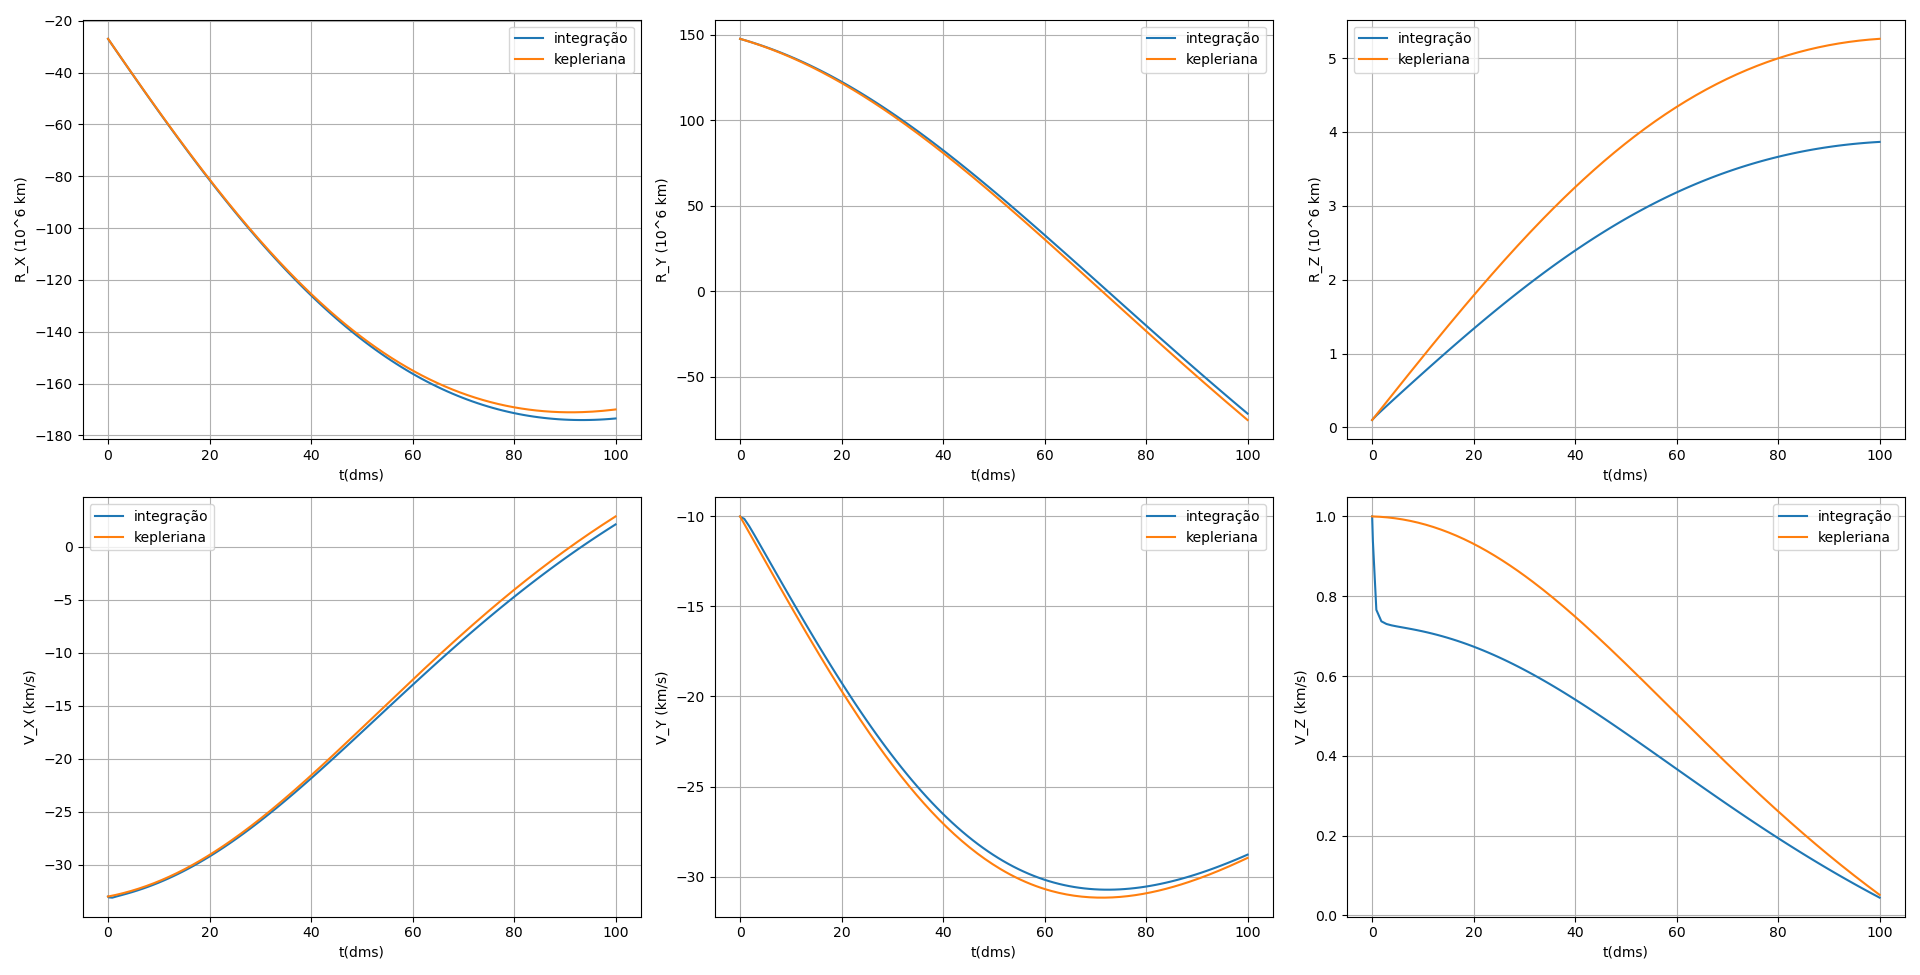
\includegraphics[width=1\textwidth]{figuras/Resultados/ex6.2.png}
\fonte{Autores, 2023}
\end{figure}

A posição inicial da espaçonave está claramente dentro do espaço de influência da terra. No entanto, devido a alta velocidade, a esfera de influência será cruzada nos próximos dias resultando em uma diminuição dessa influência. Conforme a figura \ref{fig: 1231} nota-se que para um espaço de tempo curto a perturbação que é a principal direção de ação da perturbação. conforme maior o tempo considerado maior a diferença entre os modelos evidenciando a impacto das perturbações.

\section{Problema de 3 corpos restrito}
\par Aqui é apresentada a simulação da trajetória de uma espaçonave que passa pelo ponto (0.1,0) no sistema Terra-Lua. Foram simulados os seguintes casos mostrados na tabela abaixo:

\begin{table}[h]
\centering
\caption{Componentes de Velocidade Relativa}
\label{tab:my-table}
\begin{tabular}{|l|l|l|}
\hline
Caso & $\dot{x}$ & $\dot{y}$ \\ \hline
a)    & 0         & 0.5       \\ \hline
b)    & -4        & 1         \\ \hline
c)    & -3.35     & 3         \\ \hline
d)    & -3.37     & 3         \\ \hline
e)    & -3.4      & 3         \\ \hline
f)    & -3.5      & 3         \\ \hline
g)    & -3.6      & 3         \\ \hline
\end{tabular}
\end{table}


Os resultados obtidos podem ser vistos nas figuras a seguir. Destaca-se que os resultados encontrados ficaram ligeiramente diferentes dos obtidos por \cite{book:226549}. Os autores acreditam que a divergência se dá devido ao solver utilizado. No caso deste trabalho foi utilizado o solver \textit{$solve_{ivp}$} com o método "RK45". Já \cite{book:226549} utiliza o solver ODE45 do \textit{Matlab}.


A trajetória para o caso (a) é simulada com um tempo máximo de t = 1  e é ilustrada na figura \ref{fig: cuzao } abaixo. As órbitas em torno da Terra, com rotação apsidal e nodal do plano orbital causada pela gravidade da lua ficam claras na imagem.

\begin{figure}[H]
\centering
\caption{Caso a}
\label{fig: cuzao}
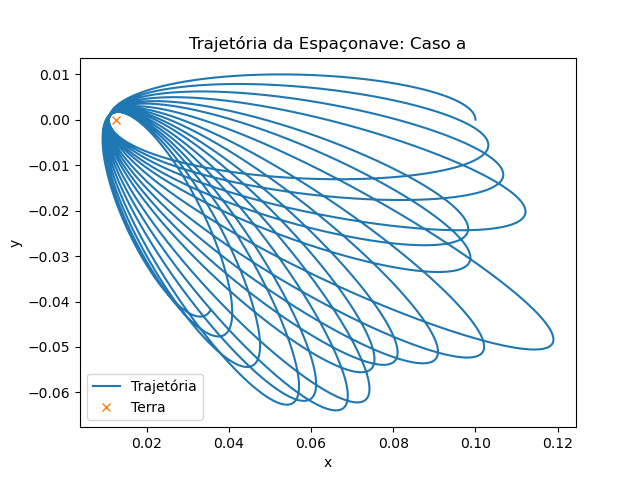
\includegraphics[width=1\textwidth]{figuras/Resultados/7.3/73casoa.png}
\fonte{Autores, 2023}
\end{figure}

\par Com o aumento da velocidade inicial para o caso (b), as órbitas em torno da Terra transformam-se em trajetórias mais energéticas e altamente excêntricas, mesmo assim o veículo  não consegue atravessar o contorno de velocidade zero de C para uma missão lunar. A figura \ref{fig: casobbb} ilustra
o decaimento da órbita com o tempo devido à gravitação da Lua.

\begin{figure}[H]
\centering
\caption{Caso b}
\label{fig: casobbb}
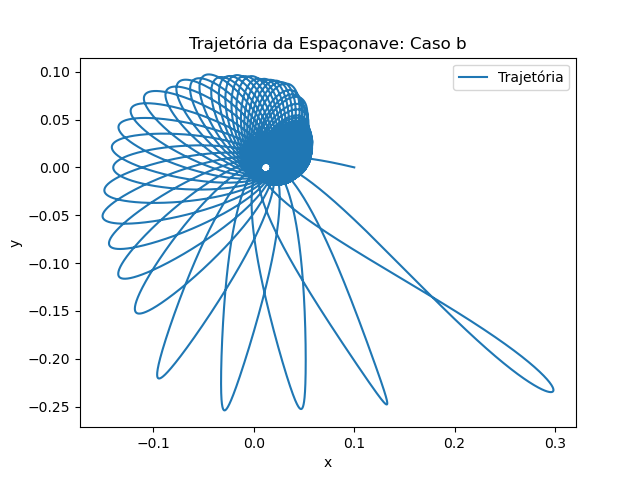
\includegraphics[width=1\textwidth]{figuras/Resultados/7.3/73casob.png}
\fonte{Autores, 2023}
\end{figure}

\par A velocidade inicial do caso (c) é suficientemente grande para uma trajetória de "regresso livre" da Lua para a terra. Neste caso, a nave espacial passa ligeiramente abaixo da órbita da Lua em torno da Terra.

\begin{figure}[H]
\centering
\caption{}
\label{fig: caso c }
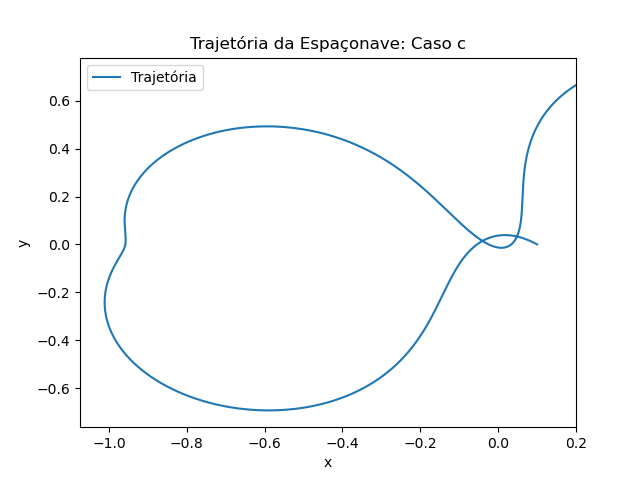
\includegraphics[width=1\textwidth]{figuras/Resultados/7.3/73casoc.png}
\fonte{Autores, 2023}
\end{figure}

\par O tempo total de voo é reduzido significativamente no caso (d) para cerca de t = 2,8, quando a nave espacial passa no entorno da Lua, entre L1 e L2. No processo, a trajetória de regresso tem uma energia cinética ligeiramente maior devido ao impulso dado pelo "estilingue" lunar . As trajetórias lunares de passagem têm sido utilizadas para para impulsionar várias naves espaciais para os pontos lagrangianos sol-terra.

\begin{figure}[H]
\centering
\caption{Caso c}
\label{fig: }
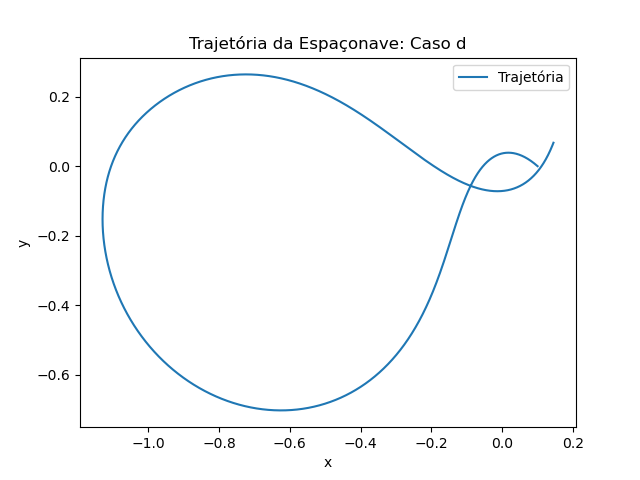
\includegraphics[width=1\textwidth]{figuras/Resultados/7.3/73casod.png}
\fonte{Autores, 2023}
\end{figure}

 No caso (e) , o tempo de voo cresce para cerca de
 t = 3.45 para uma volta completa, uma vez que a espaçonave passa mais longe da lua, passando depois do ponto L1.


\begin{figure}[H]
\centering
\caption{Caso d}
\label{fig: }
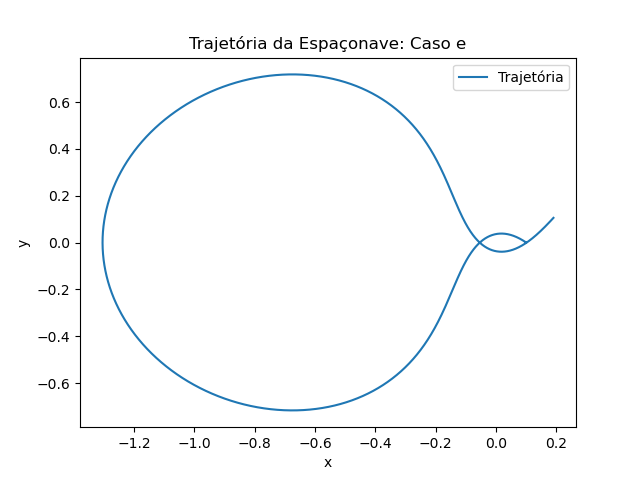
\includegraphics[width=1\textwidth]{figuras/Resultados/7.3/73casoe.png}
\fonte{Autores, 2023}
\end{figure}

Para os casos $f$ e $g$, figuras \ref{fig: f} e \ref{fig: g} respectivamente, há diferenças qualitativas nas trajetórias. é observado que para um longo tempo o caso $f$ demonstra que a espaçonave faz uma passagem pela lua a uma grande distância de $L_1$, porém é incapaz de escapar da gravidade terrestre, fazendo se aproximar mais da lua na próxima passagem, conforme mais passagens ocorrem a espaçonave é trazida para a órbita da terra com um decrescimento do raio. O caso $f$ ilustra um método mais barato para trazer um satélite para uma órbita geossíncrona, através de múltiplas passagens através da lua. Um método similar é encontrado para múltiplas passagens em planetas para diminuir o custo de missões interplanetárias.

Conforme ocorre o aumento da energia inicial para o caso $g$, a espaçonave não retorna para terra e sim embarca em uma trajetória de escape do sistema terra-lua. Nessa trajetória, a vantagem encontra-se na ajuda recebida pela gravidade lunar reduzindo o consumo de combustível e consequentemente o custo de missões interplanetárias.

\begin{figure}[H]
\centering
\caption{Caso f}
\label{fig: f}
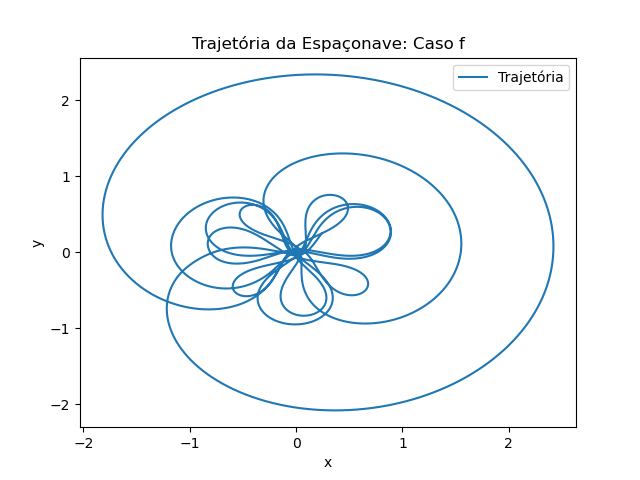
\includegraphics[width=1\textwidth]{figuras/Resultados/7.3/73casof.png}
\fonte{Autores, 2023}
\end{figure}

\begin{figure}[H]
\centering
\caption{Caso g}
\label{fig: g}
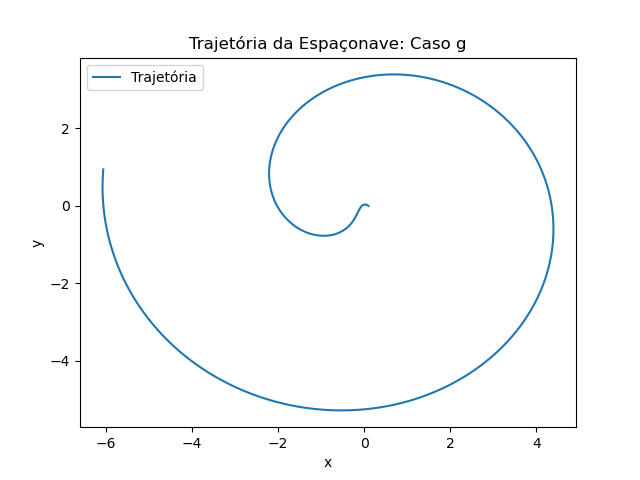
\includegraphics[width=1\textwidth]{figuras/Resultados/7.3/73casog.png}
\fonte{Autores, 2023}
\end{figure}